\chapter{Evaluierung}
\label{chap:eval}
\todo[size=\small, inline]{Walkthrough-Pfad noch einfügen hier}%
\todo[size=\small, color=yellow!40, inline]{Needs Human proofreading}%

Um die Effektivität des in dieser Arbeit entstandenen Systems überprüfen zu können, wurden verschiedene Tests durchgeführt.
Beim ersten Test, dem \textit{FPS-Test}, wurde die gemessene Bildrate bei einem Walkthrough durch die Szene aufgezeichnet. Der \textit{Reload-Test} hat bei verschiedenen Systemkonfigurationen an festen Kamerapositionen die Zeit gemessen, die ein erneutes Laden der Szene benötigt. Beim \textit{$c$-Collision-Test} wurde die Last der einzelnen Datenknoten während eines Walkthroughs gemessen. Die einzelnen Testläufe unterscheiden sich dabei in der verwendeten Anzahl an Datenknoten und Redundanzen. Redundanz bedeutet hier, wie oft das Modell der Boeing vollständig im Netzwerk verteilt wurde. \\
Zur Entwicklung des Systems wurde ein kleinerer Cluster benutzt, bestehend aus 8 Pentium Multicore-Rechnern in einem Gigabit Netzwerk, sowie einem Quadcore-Pentium mit einer GeForce 260GTX Grafikkarte als Render- und Masterknoten, im Folgenden \textit{Entwicklungs-Cluster} genannt. Die eigentlichen Tests erfolgten auf dem Arminius-Cluster des PC$^2$s (siehe Tabelle \ref{tab:impl:arminius}).\\
Im Arminius-Cluster wurde der Compiler gcc v3.4.6, OpenGL als Grafik-API, nVidia Treiber v177 auf den Rechenknoten und v190 auf den Visualisierungsknoten benutzt, sowie die boost-Bibliothek v1.38 und OpenMPI v1.2.9. Die Auflösung betrug jeweils 640$\times$480 Pixel für das normale Frustum und 800$\times$600 Pixel für das erweiterte Frustum.\\
Zusätzliche Diagramme und Abbildungen sind in den Anhängen \ref{chap:add_diag} und \ref{chap:add_fig} zu finden.

\section{FPS-Test}
\label{sec:eval:fps}
Bei diesem Test wurde in einem festgelegten Walkthrough durch die 3D-Szene gemessen, wie viele Bilder pro Sekunde an welcher Stelle der Szene erreicht werden konnten. Dazu wurde der Walkthrough auf je 24, 28 und 32 Datenknoten mit einer Redundanz von 1, 2 und 3 durchgeführt. Die y-Achsen der Diagramme in Abbildung \ref{fig:eval:fps} stellen die Bilder pro Sekunde dar und die x-Achsen die Messpunkte während des Walkthroughs. Die FPS jeden Frame darzustellen ist nicht praktikabel, da diese stark schwanken. Daher wurden die gemessenen FPS in diesem Test jeweils über 20 Frames gemittelt.
\begin{figure}
\centering
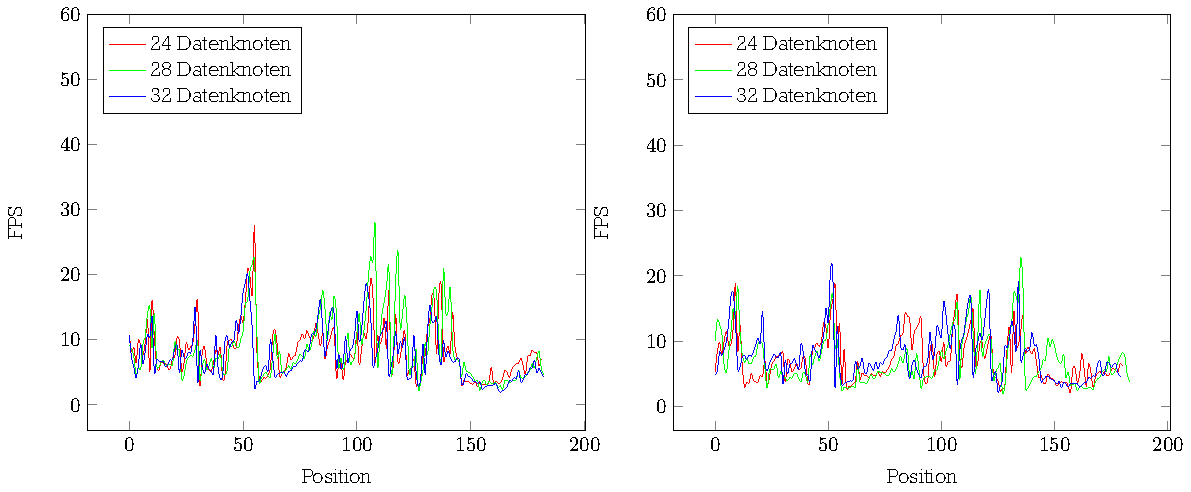
\includegraphics[scale=0.75]{images/diag_fps.pdf}
  \caption{\label{fig:eval:fps}FPS in einem Walkthrough mit 4 Renderknoten und 24-32 Datenknoten. \textit{links: Redundanz$=$1; rechts: Redundanz$=$3.}}
\end{figure}

An den Diagrammen kann man sehen, dass sich die Bildrate bei verschiedenen Konfigurationen ähnelt. Allerdings lassen sich keine Zusammenhänge zwischen Bildrate und Redundanz oder Knotenanzahl herstellen. Die Bildrate gibt eher Rückschlüsse darauf, wie die Szene an den einzelnen Positionen beschaffen ist. An Stellen des Modells, wo sehr viel Geometrie angefordert werden muss, ist die Bildrate vermutlich geringer, als an Stellen, an denen weniger angefordert wird. Hinzu kommt der Umstand, dass die Grafikkarten der Datenknoten im hier verwendeten Arminius-Cluster, nicht sehr leistungsstark sind. In Testumgebungen mit aktuellerer Grafikhardware würde die Zahl der Redundanzen und der Knoten möglicherweise stärker ins Gewicht fallen. Trotz geringerer Netzwerk-Bandbreite konnten im \textit{Entwicklungs-Cluster} teilweise höhere FPS gemessen werden, als im Arminius-Cluster. Beim gleichen Walkthrough auf dem \textit{Entwicklungs-Cluster} zeigte sich, dass nach kurzer Zeit kaum noch Objekte dargestellt wurden. Durch die kontinuierliche Bewegung wird der Tiefenbuffer alle 20 Frames aktualisiert, was zur Folge hat, dass alle laufenden Aufträge verworfen werden. In dem langsameren Netzwerk kamen dadurch kaum noch Objekte bei den Renderknoten an. Die Geschwindigkeit des verwendeten Netzwerks hat somit Auswirkungen auf die Bildqualität.

\section{Reload-Test}
\label{sec:eval:reload}
Beim Reload-Test wurde an festgelegten Kamerapositionen gemessen, wie lange die einzelnen Datenknoten benötigen, um die für diese Szene anfallenden Aufträge vollständig zu bearbeiten. Dazu wurden sämtliche auf den Renderern befindlichen Objekte verworfen und erneut angefordert. War ein Datenknoten mit der Bearbeitung aller Aufträge fertig, hat er sich beim Masterknoten zurückgemeldet und die gemessene Zeit wurde gespeichert.
\begin{figure}
\centering
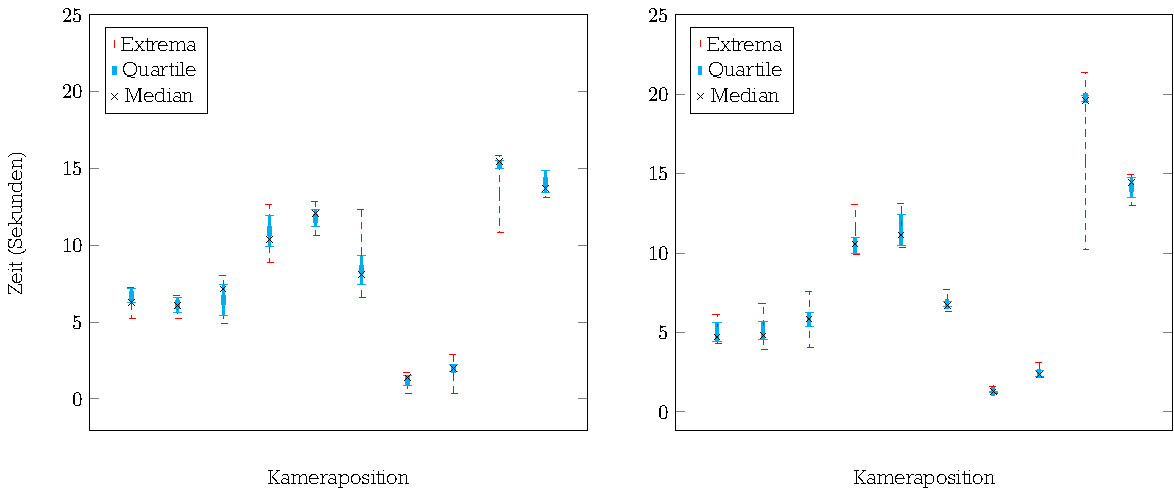
\includegraphics[scale=0.75]{images/diag_reload.pdf}
  \caption{\label{fig:eval:reload}Reload-Test mit 2 Renderknoten: \textit{links: Redundanz 1 und 24 Renderknoten; rechts: Redundanz 3 und 32 Renderknoten}.}
\end{figure}
Die Diagramme in Abbildung \ref{fig:eval:reload} enthalten auf den x-Achsen die Kameraposition und auf den y-Achsen die Render-Zeit in Sekunden. In den Diagrammen ist zu erkennen, dass der Median meist nahe am Durchschnitt liegt. Die Messungen wurden dabei mehrfach durchgeführt und die Ergebnisse wurden gemittelt. Ab und zu sind zwar einige Ausreißer zu erkennen, aber selbst die 0.25 und 0.75 Quantile liegen meist sehr dicht am Median. Das bedeutet, dass das System gut balanciert. Nur wenige Knoten benötigen mehr Zeit zum Rendern ihrer Aufträge, als das beim Median der Fall ist. Jedoch lässt auch dieser Test keinen Zusammenhang zwischen Redundanzen, Knotenanzahl und der benötigten Zeit erkennen. Die Beschaffenheit der Szene an einer gegebenen Kameraposition scheint ausschlaggebend für die gesamte benötigte Bearbeitungszeit zu sein. Mehr Geometrie an einer Position bedeutet auch mehr zu vergebene Aufträge, was mehr Zeit in Anspruch nimmt, als das bei weniger Geometrie der Fall ist. In den Abbildungen \ref{fig:eval:pos3} und \ref{fig:eval:pos5} finden sich Screenshots von zwei exemplarischen Kamerapositionen. Zusätzliche Screenshots sind im Anhang \ref{chap:add_fig} zu finden.
\begin{figure}
\centering
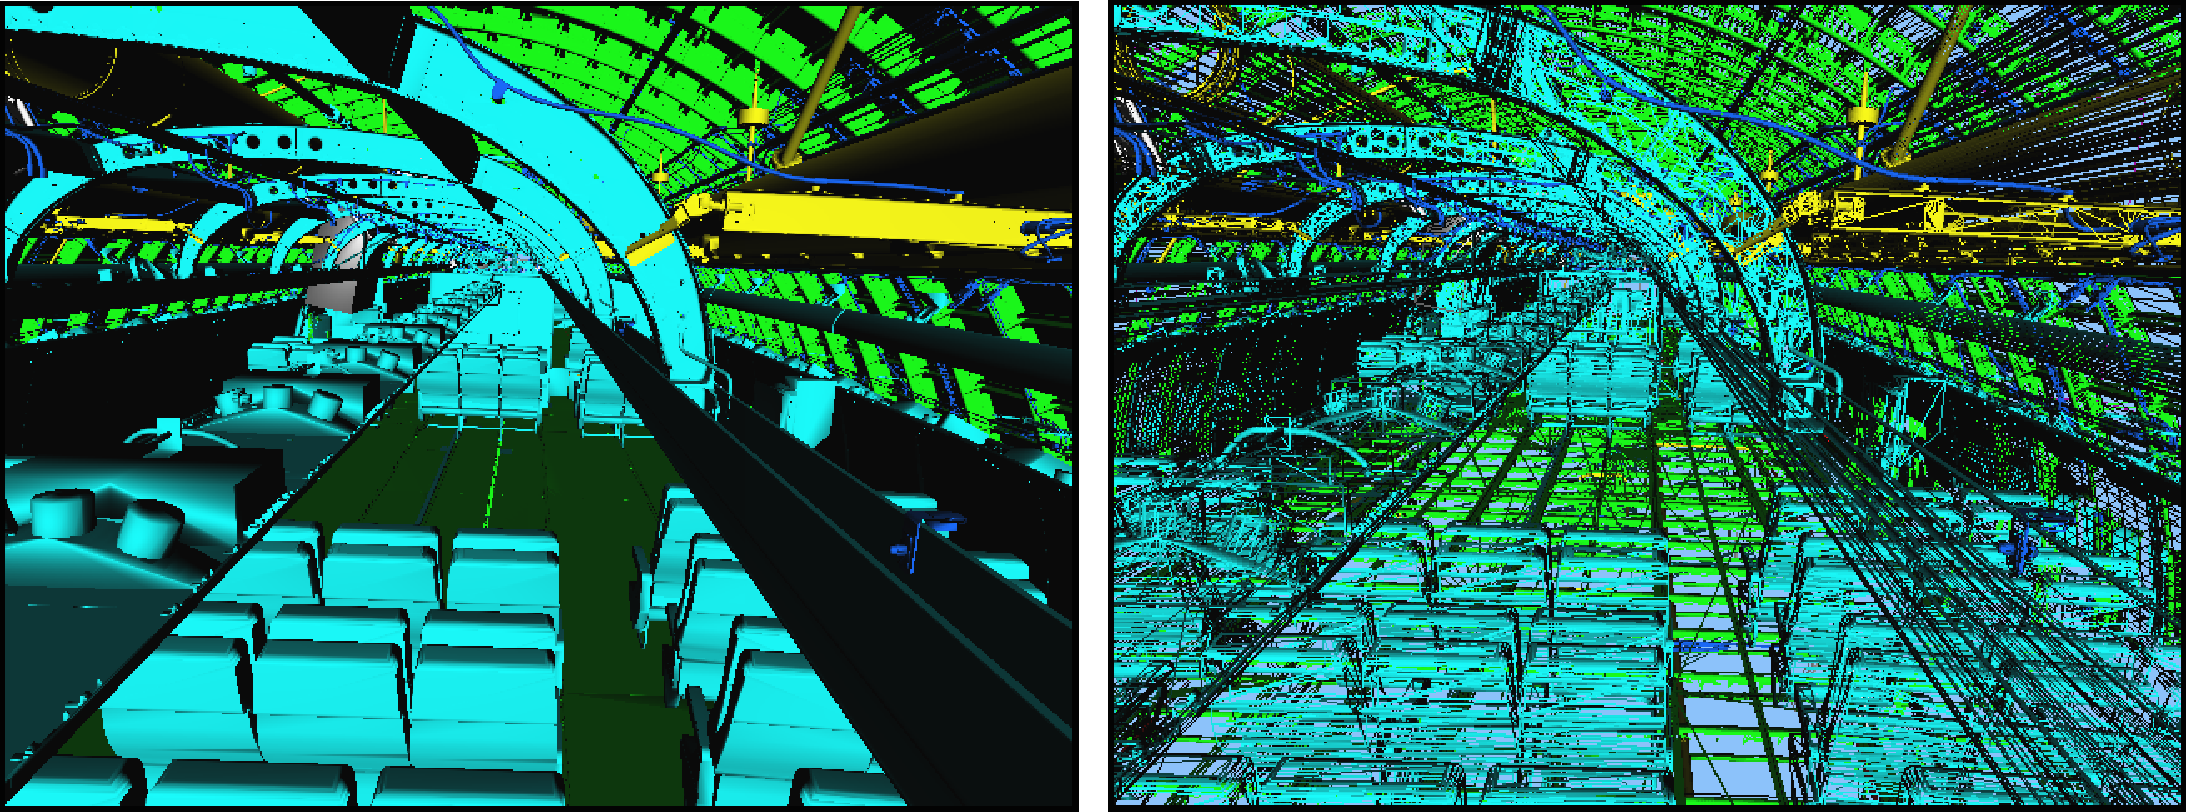
\includegraphics[scale=0.40]{images/pos3.pdf}
\caption{\label{fig:eval:pos3}Kameraposition 3: \textit{links: die Szene im normalen Rendering-Modus; rechts: die Szene im Gitternetz-Modus (Passagierbereich, 3.749.977 sichtbare Dreiecke).}}
\end{figure}

\begin{figure}
\centering
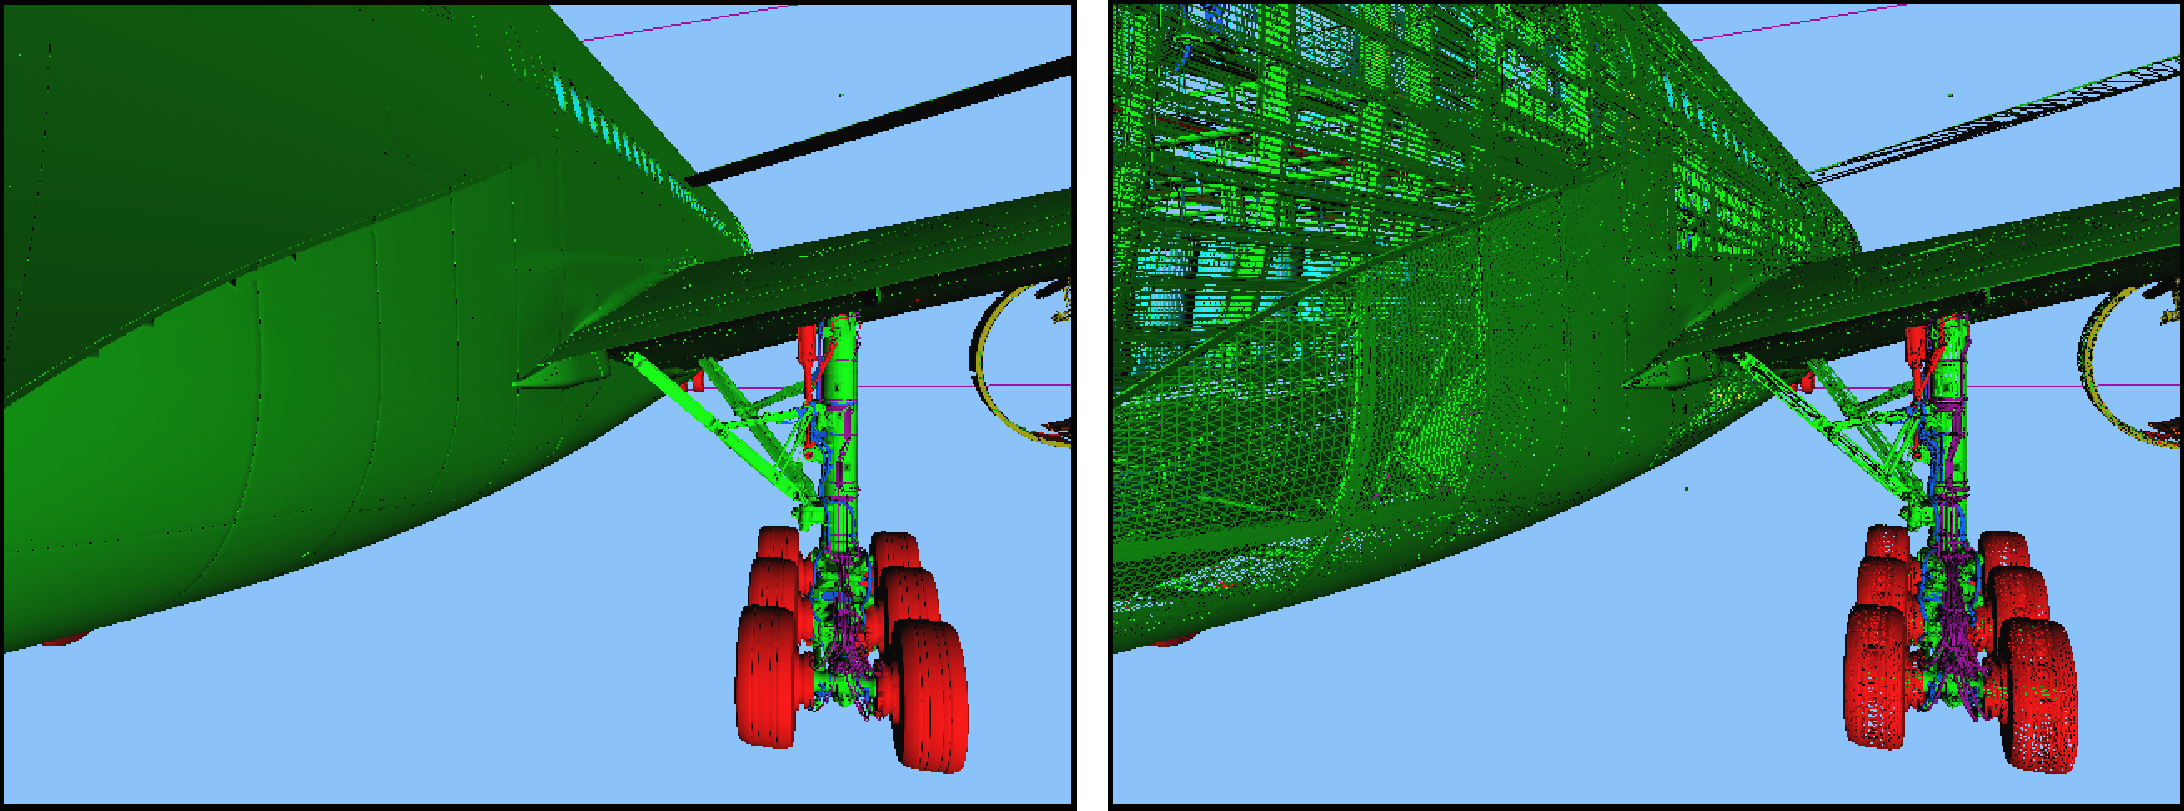
\includegraphics[scale=0.40]{images/pos5.pdf}
\caption{\label{fig:eval:pos5}Kameraposition 5 \textit{links: die Szene im normalen Rendering-Modus; rechts: die Szene im Gitternetz-Modus (Fahrwerk/Flügel, 5.776.159 sichtbare Dreiecke).}}
\end{figure}

\section{\textit{c}-Collision-Test}
\label{sec:eval:ccollision}

Der Test für das $c$-Collision Protokoll wurde als Einziger nicht im Cluster durchgeführt, sondern ausschließlich in einer Simulation. Dafür wurden alle Anfragen bei einem tatsächlichen Walkthrough durch die Szene aufgezeichnet, unmittelbar bevor sie durch das $c$-Collision Protokoll vergeben wurden. Anschließend wurden diese Aufzeichnungen genutzt, um eine beliebige Datenknotenmenge zu simulieren. Im Arminius-Cluster standen für diese Arbeit maximal 2 Visualisierungsknoten und 32 Datenknoten zur Verfügung, weshalb die Menge der Datenknoten in dieser Simulation erhöht wurde. Andere Mengen an Renderknoten lassen sich nicht ohne Weiteres simulieren, da die Renderknoten bestimmen, wann welche Objekte benötigt werden. Deshalb sind keine realistischen Aussagen über Anfragefolgen bei künstlich veränderter Renderknotenmenge möglich.\\
In diesem Test wurden 24, 80 und 120 Datenknoten simuliert. Dabei wurde die Last in Form von Dreiecken gemessen, die in jedem Frame an jeden Datenknoten vergeben wurde. In diesem Test wurden verschiedene Zufalls-Seeds benutzt und das Ergebnis wurde gemittelt.
\begin{figure}
\centering
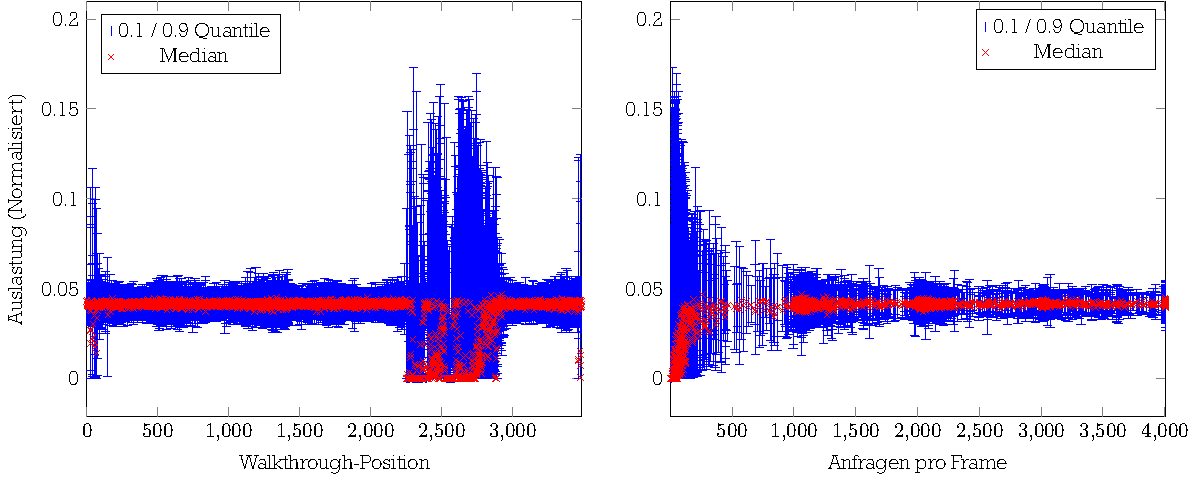
\includegraphics[scale=0.75]{images/diag_cCol_red1_render4_data24_2x.pdf}
  \caption{\label{fig:eval:cCol1}Die Auslastung der Datenknoten in einem Walkthrough bei 4 Renderknoten und 24 Datenknoten und Redundanz$=$1.}
\end{figure}

In den Abbildungen \ref{fig:eval:cCol1} und \ref{fig:eval:cCol9} zeigt das linke Diagramm jeweils die Walkthrough-Position (x-Achse) in Relation zur Lastverteilung (y-Achse). Das rechte Diagramm zeigt jeweils die Anfragenmenge, die durch das $c$-Collision Protokoll pro Frame verteilt wurde (x-Achse), in Relation zur Lastverteilung (y-Achse). In Abbildung \ref{fig:eval:cCol1} wurden 24 Datenknoten mit einer Redundanz von 1 simuliert, in Abbildung \ref{fig:eval:cCol9} wurden 120 Datenknoten mit einer Redundanz von 3 simuliert. Bei Betrachtung des linken Diagramms fallen einige Positionen auf, an denen die Last sehr ungleich verteilt ist oder der Median 0 ist. Im rechten Diagramm kann man sehen, dass dies immer dann der Fall ist, wenn das c-Collision Protkoll sehr wenige Anfragen verteilen musste. Dieses Protokoll dient ursprünglich dazu, Bälle möglichst gleichmäßig auf Körbe zu verteilen. Hat man viel weniger Bälle als Körbe, ist das System nicht gleichmäßig balanciert, da einige Körbe gar keine Bälle erhalten. Sowie die Bälle sind auch die Anfragen im Test-System atomar und werden nicht weiter unterteilt. Je nach initialer Zufallsverteilung der Daten auf den Knoten, kann es bei wenig Redundanzen auch vorkommen, dass die Aufträge nur auf wenige Knoten verteilt werden können. Im Falle des benutzen Walkthroughs, treten die unbalancierten Stellen da auf, wo das Model betreten und verlassen wird. An diesen Stellen gibt es sehr wenig sichtbare Geometrie.\\
Bei diesem Test ist zu erkennen, dass sowohl die Menge an Knoten als auch die Zahl der Redundanzen eine Rolle bei der gleichmäßigen Lastverteilung spielt. Bei erhöhter Redundanz ist zu beobachten, dass die 0.1 und 0.9 Quantile sehr viel näher am Median liegen als bei geringerer Redundanz. Mehr Datenknoten sorgen dafür, dass die Spitzenwerte an unbalancierten Stellen geringer ausfallen.
\begin{Bild}
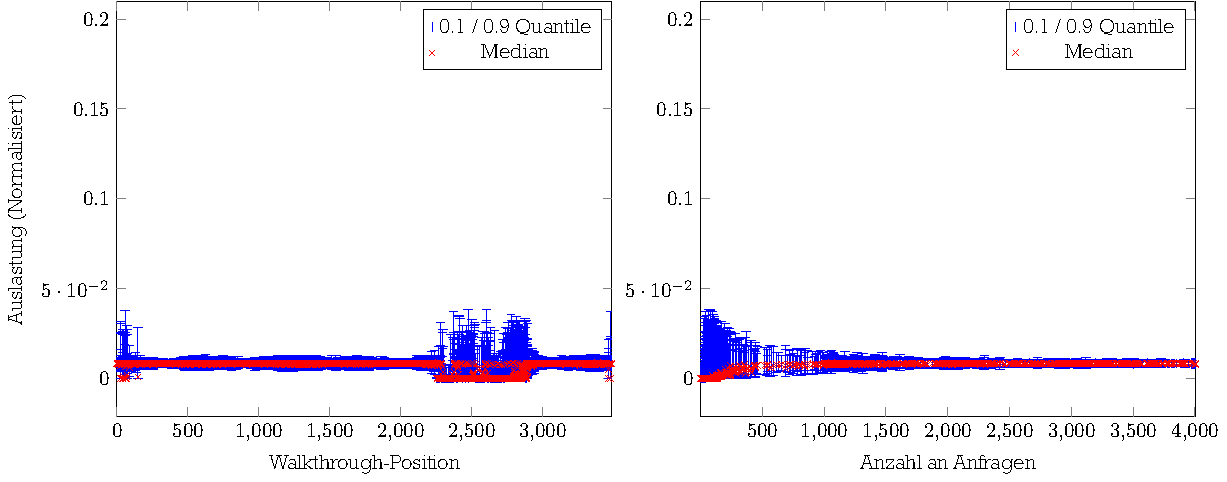
\includegraphics[scale=0.75]{images/diag_cCol_red3_render4_data120_2x.pdf}
  \captionof{figure}{\label{fig:eval:cCol9}Die Auslastung der Datenknoten in einem Walkthrough bei 4 Renderknoten und 120 Datenknoten und Redundanz$=$3.}
\end{Bild}

